\documentclass[12pt,a4paper]{article}
\usepackage[portuguese]{babel}
\usepackage[utf8]{inputenc}
\usepackage{amsmath}
\usepackage{mathrsfs}
\usepackage{amsfonts}
\usepackage{hyperref}
\usepackage{minted}
\usepackage{xcolor}
\usepackage{caption}
\usepackage{graphicx}
\usepackage{mdframed}
\usepackage{float}
\usepackage{pgfplots}
\usepackage{tikz}
\newenvironment{code}{\captionsetup{type=listing}}{}
\begin{document}
\newcommand*{\plogo}{\fbox{$\mathcal{ICMC}$}} % Generic publisher logo

%----------------------------------------------------------------------------------------
%	TITLE PAGE
%----------------------------------------------------------------------------------------

\newcommand*{\titleGP}{\begingroup % Create the command for including the title page in the document
\centering % Center all text
\vspace*{\baselineskip} % White space at the top of the page

\rule{\textwidth}{1.6pt}\vspace*{-\baselineskip}\vspace*{2pt} % Thick horizontal line
\rule{\textwidth}{0.4pt}\\[\baselineskip] % Thin horizontal line

{\LARGE SCC0630\\ Inteligência Artificial\\[0.5\baselineskip] Buscas Cega e Informada}\\[0.2\baselineskip] % Title

\rule{\textwidth}{0.4pt}\vspace*{-\baselineskip}\vspace{3.2pt} % Thin horizontal line
\rule{\textwidth}{1.6pt}\\[\baselineskip] % Thick horizontal line

\scshape % Small caps
Problema do caxeiro viajante (\emph{TSP})\\ % Tagline(s) or further description
em uma aplicação Web usando \\ % Tagline(s) or further description
Google Maps API, Prolog e Python\par % Location and year

\vspace*{2\baselineskip} % Whitespace between location/year and editors

Feito por\\[\baselineskip]
{\Large Pedro Morello Abbud\\ 
Kollins Gabriel Lima 	\\	
Carla Nunes da Cruz 	\\
Gustavo José Pereira Leite \\	
Pedro Henrique Fini 		\par} % Editor list

\vfill % Whitespace between editor names and publisher logo
{\itshape Universidade de\\ São Paulo\par} % Editor affiliation

\vfill % Whitespace between editor names and publisher logo

\plogo \\[0.3\baselineskip] % Publisher logo
{\scshape 2017} \\[0.3\baselineskip] % Year published

\endgroup}
\titleGP
\newpage
\section{Introdução}
Este trabalho foi desenvolvido para a disciplina SCC0630, Inteligência Artificial, ministrada pela Professora Solange Oliveira Rezende. O objetivo deste é aprofundar e confirmar o conhecimento de nós , alunos, acerca de buscas cegas e buscas informadas, assim como modelagem e solução de problemas. Como o projeto tem também viés didático, escolhemos utilizar a linguagem \emph{Prolog} como seu motor principal, pois esta foi a linguagem de programação de escolha nas aulas ministradas da disciplina. Dividimos a documentação e desenvolvimento deste projeto em três seções:
\begin{description}
  \item [Modelagem do Problema:]

Consiste em como definimos o problema e analisamos suas dificuldades.
\item [Solução do Problema:]

Como  foi abordado e resolvido o problema.
\item[Apresentacao do Problema:]

Escolhas para apresentar de forma clara, coerente e interessante os resultados obtidos.  
\end{description}

Foi escolhido para este projeto o problema do caixeiro-viajante, ou em inglês, \emph{TSP}, Travelling Salesman Problem.
Este é um problema clássico em computação: dado um mapa e um número de cidades, encontrar o caminho de menor distância para percorrer todas as cidades,
passando uma única vez por cada uma delas. O problema do caixeiro-viajante é um problema de alta complexidade computacional e encontrar a solução ótima para um número elevado de cidades é muito custoso.\\
De uma forma formal, podemos dizer que o problema se resume em achar o menor caminho hamiltoniano em um grafo, o que caracteriza um problema NP-Difícil.

Neste trabalho, é analisado o uso de dois métodos de busca não informada (busca em profundidade e em largura) e um método de busca informada (A*) para a solução do problema.

O problema abordado neste trabalho foi modificado em, relação ao problema original, para simplificar as implementações. As modificações feitas foram:
\begin{itemize}
  \item 

É definida uma cidade inicial, informada no início do programa para fazer a busca;
\item A busca é feita sem considerar o retorno à cidade original.
\end{itemize}

Ao longo deste documento usaremos algumas definições:
\begin{description}
  \item 
    [Estados:] Um estado é o caminho percorrido da cidade inicial até a cidade atual (com exceção do estado inicial, que não possui caminho mas apenas a cidade inicial).

  \item[Transição:] Viagem de uma cidade para a outra.

  \item [Estado final:] Caminho percorrido depois de visitar todas as cidades uma única vez (e que apresenta o menor custo).

\item [Custo:] Distância entre as cidades.

\end{description}
	
\newpage

\section{Modelagem}

\begin{figure}[htpb]
  \centering
  % Graphic for TeX using PGF
% Title: C:\Users\Carla sama\Pictures\Diagrama1.dia
% Creator: Dia v0.97.2
% CreationDate: Mon May 15 22:11:25 2017
% For: Carla sama
% \usepackage{tikz}
% The following commands are not supported in PSTricks at present
% We define them conditionally, so when they are implemented,
% this pgf file will use them.
\ifx\du\undefined
  \newlength{\du}
\fi
\setlength{\du}{15\unitlength}
\begin{tikzpicture}
\pgftransformxscale{1.000000}
\pgftransformyscale{-1.000000}
\definecolor{dialinecolor}{rgb}{0.000000, 0.000000, 0.000000}
\pgfsetstrokecolor{dialinecolor}
\definecolor{dialinecolor}{rgb}{1.000000, 1.000000, 1.000000}
\pgfsetfillcolor{dialinecolor}
\definecolor{dialinecolor}{rgb}{1.000000, 1.000000, 1.000000}
\pgfsetfillcolor{dialinecolor}
\pgfpathellipse{\pgfpoint{18.896664\du}{6.598322\du}}{\pgfpoint{3.153364\du}{0\du}}{\pgfpoint{0\du}{3.101682\du}}
\pgfusepath{fill}
\pgfsetlinewidth{0.100000\du}
\pgfsetdash{}{0pt}
\pgfsetdash{}{0pt}
\pgfsetmiterjoin
\definecolor{dialinecolor}{rgb}{0.000000, 0.000000, 0.000000}
\pgfsetstrokecolor{dialinecolor}
\pgfpathellipse{\pgfpoint{18.896664\du}{6.598322\du}}{\pgfpoint{3.153364\du}{0\du}}{\pgfpoint{0\du}{3.101682\du}}
\pgfusepath{stroke}
% setfont left to latex
\definecolor{dialinecolor}{rgb}{0.000000, 0.000000, 0.000000}
\pgfsetstrokecolor{dialinecolor}
\node at (18.896664\du,6.838322\du){Cidade de Origem};
\definecolor{dialinecolor}{rgb}{1.000000, 1.000000, 1.000000}
\pgfsetfillcolor{dialinecolor}
\pgfpathellipse{\pgfpoint{19.271642\du}{18.373286\du}}{\pgfpoint{3.064942\du}{0\du}}{\pgfpoint{0\du}{3.121286\du}}
\pgfusepath{fill}
\pgfsetlinewidth{0.100000\du}
\pgfsetdash{}{0pt}
\pgfsetdash{}{0pt}
\pgfsetmiterjoin
\definecolor{dialinecolor}{rgb}{0.000000, 0.000000, 0.000000}
\pgfsetstrokecolor{dialinecolor}
\pgfpathellipse{\pgfpoint{19.271642\du}{18.373286\du}}{\pgfpoint{3.064942\du}{0\du}}{\pgfpoint{0\du}{3.121286\du}}
\pgfusepath{stroke}
% setfont left to latex
\definecolor{dialinecolor}{rgb}{0.000000, 0.000000, 0.000000}
\pgfsetstrokecolor{dialinecolor}
\node at (19.271642\du,18.613286\du){Cidade de Destino};
\pgfsetlinewidth{0.100000\du}
\pgfsetdash{}{0pt}
\pgfsetdash{}{0pt}
\pgfsetbuttcap
{
\definecolor{dialinecolor}{rgb}{0.000000, 0.000000, 0.000000}
\pgfsetfillcolor{dialinecolor}
% was here!!!
\pgfsetarrowsend{stealth}
\definecolor{dialinecolor}{rgb}{0.000000, 0.000000, 0.000000}
\pgfsetstrokecolor{dialinecolor}
\pgfpathmoveto{\pgfpoint{15.983534\du}{7.784643\du}}
\pgfpatharc{201}{158}{14.519509\du and 14.519509\du}
\pgfusepath{stroke}
}
\pgfsetlinewidth{0.100000\du}
\pgfsetdash{}{0pt}
\pgfsetdash{}{0pt}
\pgfsetbuttcap
{
\definecolor{dialinecolor}{rgb}{0.000000, 0.000000, 0.000000}
\pgfsetfillcolor{dialinecolor}
% was here!!!
\pgfsetarrowsend{stealth}
\definecolor{dialinecolor}{rgb}{0.000000, 0.000000, 0.000000}
\pgfsetstrokecolor{dialinecolor}
\pgfpathmoveto{\pgfpoint{22.099548\du}{17.601158\du}}
\pgfpatharc{22}{-24}{12.551604\du and 12.551604\du}
\pgfusepath{stroke}
}
% setfont left to latex
\definecolor{dialinecolor}{rgb}{0.000000, 0.000000, 0.000000}
\pgfsetstrokecolor{dialinecolor}
\node[anchor=west] at (22.950000\du,12.700000\du){Distância de Volta};
% setfont left to latex
\definecolor{dialinecolor}{rgb}{0.000000, 0.000000, 0.000000}
\pgfsetstrokecolor{dialinecolor}
\node[anchor=west] at (10.300000\du,12.700000\du){Distância de Ida};
\end{tikzpicture}

  \caption{Modelagem do problema em grafo}
  \label{fig:1}
\end{figure}

A figura \ref{fig:1} mostra uma representação das cidades e suas interligações modeladas em um grafo. Cada nó do grafo representa uma cidade e as arestas são os caminhos, cada qual possui um custo associado.

Para uma abordagem mais realista, foi utilizada a API do Google Maps em um script Python para obter as distâncias reais entre cidades reais. A partir deste script, são exportadas as regras para o prolog, onde foi feita a implementação da busca. Desta forma, pôde-se modelar o problema de forma dinâmica e interativa.

Assim, criamos uma função que se comunica com a API do Google Maps, e extraí dela uma matriz de conectividade, que indica o custo de cada transição. O código está representado no bloco de código abaixo:

  %\centering
\begin{mdframed}[linecolor=black, topline=true, bottomline=true,
  leftline=false, rightline=false, backgroundcolor=yellow!10!white]
\inputminted[tabsize=2,linenos=true,fontsize=\footnotesize,breaklines=true,breakafter=format]{python}{../DistanceMatrix.py}
\end{mdframed}
%\caption{\emph{DistanceMatrix.py} - Constrói regras de Prolog apartir da API do Google Maps}

A função \mintinline{python}{places_distance_matrix()} usa o wrapper Python do google maps e envia a lista de lugares a serem percorridos e retorna a string com a resposta da API. 

A função \mintinline{python}{extract_distance_matrix()} é apenas um filtro para a respota da API do googlemaps, que devolve a matrix de conectividade desejada.

A função  \mintinline{python}{construct_rules()} a partir da resposta já filtrada da API constrói um arquivo com fatos necessários para a execução da busca em Prolog.


\newpage
\section{Solução}
Modelado nosso problema e definido as regras, finalmente podemos começar a resolvê-lo. Desenvolvemos dois programas em Prolog que encontram o menor caminho para o TSP. O primeiro programa utiliza uma busca cega sem heurística, visitando todas as possibilidades de seu espaço de busca antes de encerrar sua execução. A segunda estratégia foi utilizar do algoritmo A* que sempre reavalia os possíveis melhores caminhos;

\subsection{Busca Cega}
Para a busca cega, foi testada tanto a busca em profundidade quanto a busca em largura para avaliar qual apresenta o melhor resultado. O código está representado no bloco abaixo:

  %\centering
\begin{mdframed}[linecolor=black, topline=true, bottomline=true,
  leftline=false, rightline=false, backgroundcolor=yellow!10!white]
\inputminted[tabsize=2,linenos=true,fontsize=\footnotesize,breaklines=true,breakafter=format]{prolog}{../buscacega_profundidade.pl}
\end{mdframed}
%\caption{\emph{buscacega\_profundidade.pl} - Define uma busca cega por profundidade}
  \label{Code:2}

\subsection{Busca Informada}
Para fazer a busca informada foi utilizada a estratégia A*. Essa estratégia foi utilizada por trabalhar com caminhos, e não apenas com um resultado final, o que é ideal para o problema. Também é interessante por não retornar um resultado aproximado, mas sim um resultado ótimo, desde que seja utilizada uma função de avaliação admissível. 
	Um ponto negativo desta estratégia é a quantidade de memória utilizada já que todos os caminhos tentados são armazenados (embora apenas um caminho esteja sendo desenvolvido por vez). Em nossos testes, não foi possível encontrar a solução para, em média, mais de 7 cidades.
  A heurística utilizada para guiar a busca A* foi a de vizinho mais próximo. Nesta, a função de avaliação é sempre zero (e portanto é admissível) e a função de custo é a distância entre as cidades. (Foi implementada também a heurística de inserção mais barata, fazendo a função de avaliação ser a distância em linha reta entre as cidades, no entanto essa apresentou uma performance pior, certamente devido à maneira como foi implementada.)
  Segue o código:

  %\centering
  \begin{mdframed}[linecolor=black, topline=true, bottomline=true,
  leftline=false, rightline=false, backgroundcolor=yellow!10!white]
\inputminted[tabsize=2,linenos=true,fontsize=\footnotesize,breaklines=true,breakafter=format]{prolog}{../buscaInformada_A.pl}
\end{mdframed}
%\caption{\emph{buscaInformada\_A.pl} - Define a busca informada A* }
  \label{Code:3}

A fim de testar e avaliar o desempenho dos algoritmos criados, desenvolvemos um programa que cria uma classe que executa todos os códigos anteriores, isto é cria as regras do caminho especificado e executa as buscas. Assim, temos de forma acessível o tempo que cada algoritmo levou para ser executado, o caminho resultante e a distância em metros que é a soma dos custos no estado final. Como o Prolog é limitado, esta comunicação foi feita a partir da criação de arquivos auxiliares. O código está representado abaixo:

  \begin{mdframed}[linecolor=black, topline=true, bottomline=true,leftline=false, rightline=false, backgroundcolor=yellow!10!white]
\inputminted[tabsize=2,linenos=true,fontsize=\footnotesize,breaklines=true,breakafter=format]{python}{../PrologIO.py}
\end{mdframed}
%\caption{\emph{PrologIO.py} Recupera os resultados das buscas feitas em Prolog}
  \label{Code:4}
\newpage
  \section{Apresentação dos resultados}
\begin{figure}[H]
  \centering
  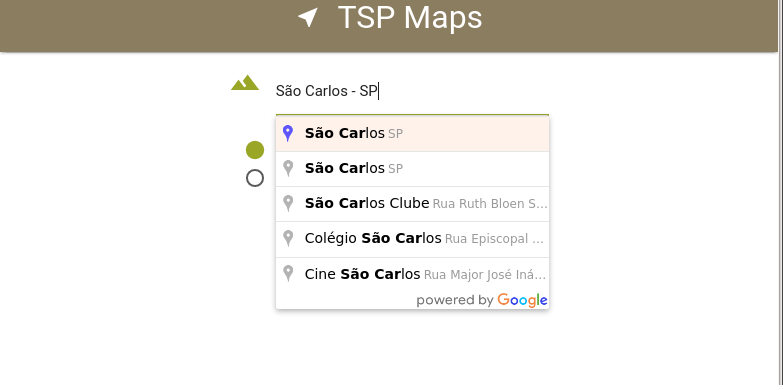
\includegraphics[width=0.8\linewidth]{tela1.png}
  \caption{Interface do usuário com autocomplete}
  \label{fig:tela1}
\end{figure}
  Como um terminal de query Prolog parece críptico, pouco intuitivo e amigável para o usuário final, escolhemos desenvoler uma aplicação Web que reutiliza-se todos os nosso códigos. Para isso, foi escolhido um micro-framework Web, em Python, chamado \emph{Flask}. Flask define rotas e executa uma função quando uma requisição \emph{HTTP} acontece. Assim, nosso código contido em \emph{PrologIO.py} executa e retorna uma página, com template predefinido por nós, renderizada com todos os dados relevantes contidos da classe \emph{ResultadosBusca}, de forma legível e amigável. O código em Flask é dado abaixo:
  \begin{mdframed}[linecolor=black, topline=true, bottomline=true,leftline=false, rightline=false, backgroundcolor=yellow!10!white]
\inputminted[tabsize=2,linenos=true,fontsize=\footnotesize,breaklines=true,breakafter=format]{python}{../tspserver.py}
\end{mdframed}

Escolhemos o framework front-end (CSS/Javascript) \emph{Materialize} para embelezar nossa aplicação.

\begin{figure}[H]
  \centering
  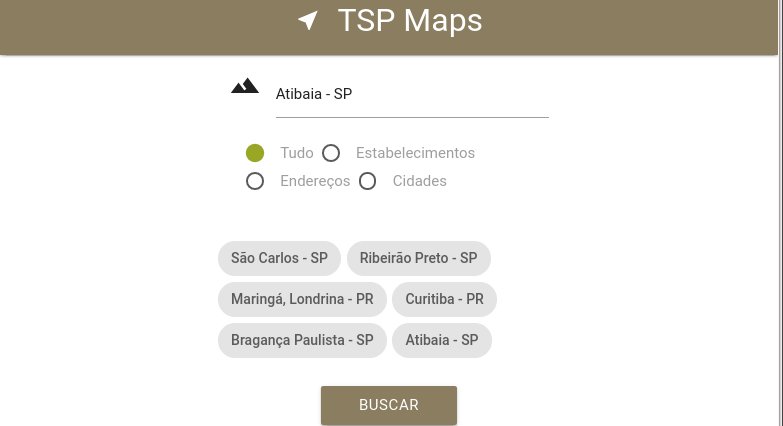
\includegraphics[width=0.8\linewidth]{tela2.png}
  \caption{Nós a se percorrer já selecionados (o primeiro selecionado é o inicial)}
  \label{fig:tela2}
\end{figure}
\begin{figure}[H]
  \centering
  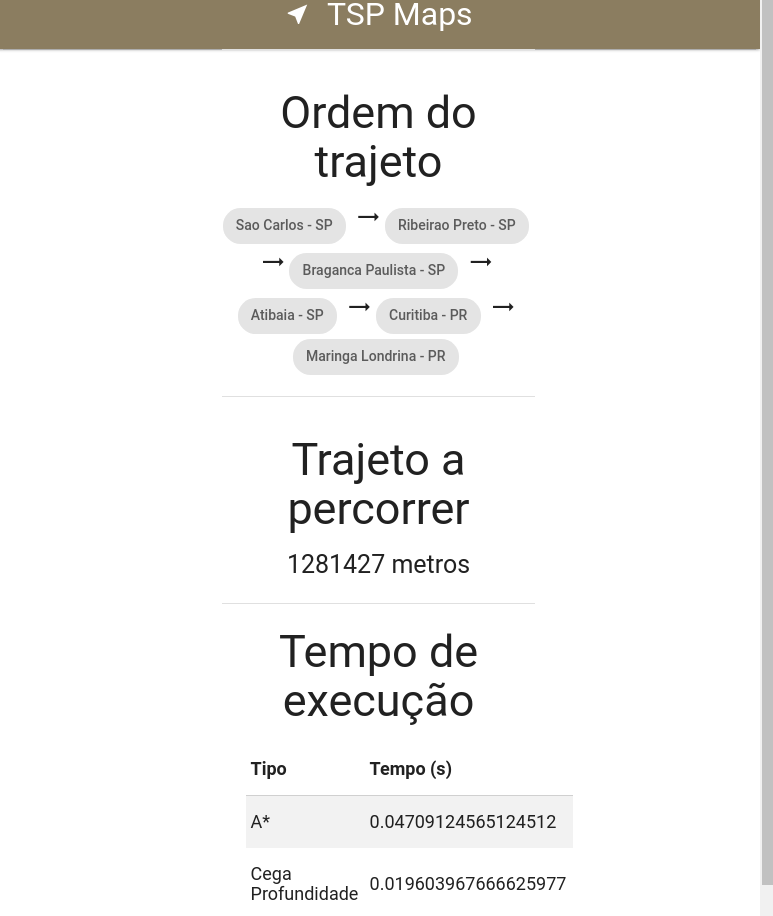
\includegraphics[width=0.8\linewidth]{tela3.png}
  \caption{Busca realizada e resultados}
  \label{fig:tela3}
\end{figure}
% \begin{figure}[ht]
%   \centering
%   \includegraphics[width=0.8\linewidth]{}
%   \caption{}
%   \label{fig:}
% \end{figure}
\section{Avaliação de Desempenho}
Após a implementação do problema do caixeiro viajante foram realizados testes para extração dos resultados para busca cega e busca informada. Os gráficos abaixo representam dois testes realizados.
\begin{figure}[ht]
  \centering
  \begin{tikzpicture}
	\begin{axis}[
    xlabel=Nós,
    ylabel=Tempo($s$)]
	\addplot[color=red,mark=x] file {teste2_ia.csv};
  \addplot[color=blue,mark=*]  file {teste22_ia.csv};
  \legend{Busca Cega Profundidade, Busca A*}
	\end{axis}
\end{tikzpicture}

  \caption{Comparação no Teste 1}
  \label{fig:2}
\end{figure}

\begin{figure}[ht]
  \centering
  \begin{tikzpicture}
	\begin{axis}[
    xlabel=Nós,
    ylabel=Tempo$(s)$]
	\addplot[color=red,mark=x] file {teste1_ia.csv};
  \addplot[color=blue,mark=*]  file {teste11_ia.csv};
  \legend{Busca Cega Profundidade, Busca A*}
	\end{axis}
\end{tikzpicture}

  \caption{Comparação no Teste 2}
  \label{fig:3}
\end{figure}

Para o primeiro teste o custo para ir de um nó a outro foi considerado igual, dessa forma, é possível observar a partir da Figura~\ref{fig:2} que a busca em profundidade tem tempo execução mais rápido que a A*, se mostrando mais vantajosa uma vez que o A* se torna um tanto complexa para problemas com poucos nós. Além disso, neste caso a busca informada A* se comporta de maneira aproximada a busca em largura.

Para o segundo teste, os custos considerados foram aleatórios para cada caminho gerando a Figura~\ref{fig:3}. Neste gráfico, o  tempo de execução dos algoritmos se inverte, a busca A* se torna mais vantajosa conforme o número de nós cresce enquanto a busca em profundidade têm tempos de execução cada vez maiores.
É ainda importante ressaltar que para ambos os testes a busca A* é limitada em razão da memória disponível.

\newpage
\section{Conclusão}
	Podemos concluir que, para o problema do caixeiro-viajante, a estratégia de busca A* pode ser muito cara pois o consumo de memória cresce muito a partir de 8 nós se não utilizar uma heurística para evitar a expansão de todos os caminhos (o limite do prolog para sistemas 64 bits, onde foi testado, é de 256Mb. Este limite foi expandido para 2GB e mesmo assim com 8 nós ocorreu falha por falta de memória no primeiro teste). A heurística utilizada (vizinho mais próximo) permitiu que o problema fosse resolvido com 9 nós.

	Quanto a busca em profundidade, ela possui uma vantagem de não ocupar tanta memória, o que permite encontrar soluções para problemas com mais nós. No entanto, o número de possibilidades a serem testadas é um grande problema (foi possível solucionar problemas com 10 nós utilizando busca em profundidade, mas o tempo gasto ultrapassava 1 minuto, o que tornou inviável fazer diversas medições para tirar uma média de tempo.)

  Assim sendo, dado que limitações de memória não estão presentes, a Busca A* se mostrou superior para muitos nós enquanto a busca em profundidade é vantajosa com problemas de pequena escala ou em ambientes com memória limitada.
\appendix

\section{Instalação e Execução}
\subsection{Instalação}
Certifique-se que Python 3+ está instalado na sua máquina:

Ubuntu-Based:
\begin{minted}{bash}
$ sudo apt-get install software-properties-common 
\end{minted}

ArchLinux:
\begin{minted}{bash}
$ sudo pacman -S python3
\end{minted}

Instale o compilador Swi Prolog, seguindo estas instruções:

\url{http://www.swi-prolog.org/Download.html}

Alternativamente no ArchLinux:
\begin{minted}{bash}
$ sudo pacman -S swi-prolog
\end{minted}

Instale o gerenciador de pacotes do Python,  \emph{Pip}, seguindo estas instruções: 

\url{https://pip.pypa.io/en/stable/installing/}

Em seguida, instale os módulos utilizados neste trabalho:
\begin{minted}{bash}
$ sudo pip install googlemaps

$ sudo pip install flask

$ sudo pip install unidecode
\end{minted}
\subsection{Execução}

Na pasta principal, defina quem é a aplicação flask:
\begin{minted}{bash}
$ export FLASK_APP=tspserver.py
\end{minted}

Rode a aplicação:
\begin{minted}{bash}
$ flask run
\end{minted}

Acesse-a via browser \url{http://127.0.0.1:5000/}.
\end{document}
